This question can be a good application of the \textit{secretary problem}. Algorithm is like that:

\begin{itemize}
  \item For $n$, we skip the predefined $k$ elements while keeping the max of the seen elements in the memory.
  \item After $k$ elements, we choose the next larger element than seen max. Here, larger element may not be seen, then we go to the end of the array and choose the last one.
\end{itemize}

Why this algorithm is correct is defined by a simple probability calculation:

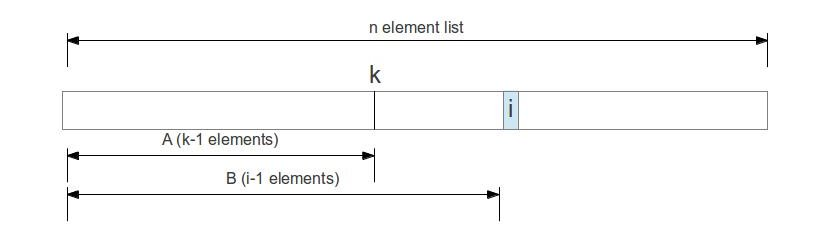
\includegraphics[scale=0.5]{q4}

  Here, we skip $k$ elements, and $i$th element is the max and we are able to choose it. If it is put into a formula:

\begin{equation*}
  P(k) = \sum_{i=1}^{n} P(\text{$i$ selected} | \text{$i$ is the best}) \cdot P(\text{$i$ is the best})
\end{equation*}

  Max element can be found at the index from $1$ to $n$ because it is just a random permutation. Therefore, having max element at the index $i$ is $\frac{1}{n}$. Moreover, since we skip the first $k$ elements, the probability of finding max in between them is zero if max is there. Therefore, above sum until $k$ doesn't contribute anything.

\begin{equation*}
  P(k) = \left( \sum_{i=1}^{k-1} 0 \cdot \frac{1}{n} \right) + \left(\sum_{i=k}^{n} P(\text{$i$ selected} | \text{$i$ is the best}) \cdot \frac{1}{n} \right)
\end{equation*}

  However, if max is following the skipped elements, then it can be found:
  
\begin{equation*}
  P(k) = \sum_{i=r}^{n} P(
         \text{the best in the first $i-1$ is among the first $k-1$} | \text{$i$ is the best}) \cdot \frac{1}{n}
\end{equation*}

  For the algorithm to be able to select $i$, that would mean that there are no other items with value greater than $i$ in the space between $k$ and $i$(B-A). Thus, there must be at least one item in $k$ with value greater than all the items before $i$. The probability of max of $i − 1$ elements(B) must be in first $k − 1$ elements(A) would be $\frac{k-1}{i-1}$. Otherwise we would choose as max a value between $k$ and $i$, not the actual max.

\begin{align*}
   P(k) &= \sum_{i=k}^{n} \frac{k-1}{i-1} \cdot \frac{1}{n} \\
        &= \frac{k-1}{n} \sum_{i=k}^{n} \frac{1}{i-1} 
\end{align*}
         
  Optimal $k$ can be found iteratively, setting it to 2 going upwards by calculating above result. When we arrive a probability larger than desired probability(0.25 in our case), algorithm stops. Then, by using found $k$, chooses probable max so skips first $k$ elements but notes down the max of them and after $k$ elements, picks the first element larger than known max.
  
  However, we can calculate a $k$ value that can work for all $n$. For example, by setting $k = \frac{n}{2}$ because $P(k)$ will always larger than 0.25 (to be specific, it is around 0.35).